% Compile: pdflatex + bibtex + pdflatex x2
\documentclass[11pt,a4paper]{article}

\usepackage[T1]{fontenc}
\usepackage[utf8]{inputenc}
\usepackage{lmodern}
\usepackage{microtype}
\usepackage[margin=1in]{geometry}
\usepackage{amsmath,amssymb,bm}
\usepackage{array}
\usepackage{booktabs}
\usepackage{graphicx}
\usepackage{xcolor}
\usepackage{hyperref}
\usepackage{natbib}
\usepackage{setspace}
\usepackage{subcaption}
\usepackage[section]{placeins}
\definecolor{linkblue}{RGB}{0,70,120}
\hypersetup{
  colorlinks=true,
  linkcolor=linkblue,
  citecolor=linkblue,
  urlcolor=linkblue
}

\graphicspath{{../output/}}

\title{\textbf{Fiscal Policy in a Stochastic Markov RBC Model}\\[0.35em]
  \large Government Spending, Ricardian Equivalence, and Evidence}
\author{National University of Singapore\\Spring 2026}
\date{April 15, 2026}

\begin{document}
\maketitle

\begin{abstract}
\noindent
This paper quantifies fiscal transmission in a neoclassical real business-cycle (RBC) economy with capital, endogenous labor, and productivity following a two-state Markov chain. The benchmark is solved by \textbf{value-function iteration} on a capital grid at each $z\in\{z_L,z_H\}$, with labor chosen conditional on next-period capital $k'$ and continuation values integrated using $\bm{\Pi}$. Fiscal impulse responses are Monte Carlo averages over stochastic future productivity paths; all quantitative results below come from a single fully documented numerical replication. An unforeseen one-quarter increase in government spending equal to $5\%$ of steady-state $g$ (about $1.0\%$ of baseline output) raises impact output by $4.752$ log points, lowers consumption by $5.077$, raises labor by $7.424$, and raises investment by $29.875$. We study three fiscal experiments, contrast $z_L$ versus $z_H$ while holding a \textbf{common absolute} one-time increment to $g$, and verify Ricardian equivalence using equilibrium bond prices $q_t=\beta\,\mathbb{E}_t[(c_{t+1}/c_t)^{-\sigma}]$, zero flow-budget residuals at reported precision, and \textbf{allocation invariance} of simulated $(c,n,k,y,g)$ across financing schemes. Empirically we use a fixed quarterly U.S.\ sample (1980Q1--2025Q4) and report a reduced-form VAR(4), HAC local projections on the recursive fiscal innovation, and \textbf{IV local projections} that instrument $\Delta\log G$ with a predetermined lag; the IV first-stage statistic at horizon $0$ is only $2.13$, so identification remains weak. Relative to our recursive estimates, the model preserves the sign of impact consumption crowding out but misses the negative impact output-hours pattern in the data. A distortionary labor-tax extension uses an auxiliary perfect-foresight stack to locate where Ricardian neutrality fails.
\vspace{0.6em}

\noindent\textbf{Keywords:} fiscal policy; Ricardian equivalence; Markov chain; value function iteration; fiscal multipliers.

\noindent\textbf{JEL Classification:} E62; E32; C63.
\end{abstract}

\onehalfspacing

\section{Introduction}

Fiscal multipliers and the financing of government purchases are central in macroeconomics, yet their quantitative magnitude and even the sign of the private consumption response remain contested across frictionless neoclassical models, reduced-form vector autoregressions (VARs), local projections, and narrative shock designs. This paper studies a stochastic Markov RBC economy: Ricardian equivalence in the lump-sum benchmark (with a pricing-based numerical check), impulse responses to three fiscal experiments, state dependence across $z_L$ and $z_H$, empirical comparison using U.S.\ quarterly data alongside canonical references, and an extension with distortionary labor taxation.

Two commitments structure the analysis. First, every number in the main text is tied to one documented numerical replication: fixed-point objects, impulse-response summaries, model--data comparisons, and appendix diagnostics are generated jointly, so tables and figures describe the same equilibrium. Second, the empirical block is a deliberate \emph{comparison exercise}: we report recursive VAR, VAR-residual local projections, and a weak-IV local projection together, because identification uncertainty is substantive for interpreting fiscal comovements.

Productivity $z_t\in\{z_L,z_H\}$ follows $\bm{\Pi}$; households maximize $\mathbb{E}_0\sum_t \beta^t[u(c_t)-v(n_t)]$ under competitive markets, with expectations in intertemporal conditions integrating over $\bm{\Pi}$ via the solved policies. Fiscal impulse responses average over Monte Carlo draws of future $z$, which is the natural rational-expectations notion in this Markov setting.

\paragraph{Main quantitative findings.}
Relative to deterministic steady state at $\bar z$, Markov rational-expectations policies imply state-contingent long-run capital with $k'(k,z)\approx k$ (Table~\ref{tab:markov_fp}). The unforeseen fiscal experiment raises $g$ by five percent of $g_{\mathrm{ss}}$ at \textbf{ergodic-mean} $\bar z$; the \textbf{same absolute} $\Delta g$ is used when comparing $z_L$ versus $z_H$. Monte Carlo means ($1200$ draws) underlie Table~\ref{tab:irf_impact} and the state-dependence summary. The one-time shock raises impact output by $4.752$ log points and labor by $7.424$, lowers consumption by $5.077$, and raises investment by $29.875$; the investment figure is large partly because $\Delta g$ is about $3.9\%$ of baseline investment, so log-percentage responses magnify. State dependence in the narrow calibration is modest for output and labor but visible: at impact, the $z_H-z_L$ gap is $0.53$ log points for output, $0.82$ for labor, and $4.12$ for investment. Appendix tables record solver and empirical diagnostics. Section~\ref{sec:empirical} contrasts Cholesky VAR, VAR-residual LP, and IV-LP with the model and the literature (Table~\ref{tab:lit}).

\paragraph{Outline.}
Sections~2--5 present the model, calibration, and numerical method. Sections~\ref{sec:ricardian}--\ref{sec:states} give fiscal results and $z_L$--$z_H$ comparisons. Section~\ref{sec:empirical} juxtaposes model moments with data and selected papers; the extension and conclusion summarize what the frictionless benchmark explains and what richer mechanisms would add.

\section{Baseline model}

\subsection{Environment}
Time is discrete. A representative household rents capital and supplies labor; a firm produces with Cobb--Douglas technology; the government purchases $g_t$, levies lump-sum taxes $\tau_t$, and issues one-period bonds. Productivity follows a first-order Markov chain. Preferences are
\begin{equation}
  \mathbb{E}_0\sum_{t=0}^{\infty}\beta^t
  \left[
    \frac{c_t^{1-\sigma}-1}{1-\sigma}
    -
    \chi\frac{n_t^{1+\phi}}{1+\phi}
  \right],
\end{equation}
with the log-utility case understood as the $\sigma\to1$ limit.

\subsection{Household and equilibrium}
The household maximizes expected discounted utility subject to
\begin{equation}
  c_t + k_{t+1} + q_t a_{t+1}
  =
  w_t n_t + \bigl(r^k_t + 1 - \delta\bigr)k_t + a_t - \tau_t,
\end{equation}
plus a standard no-Ponzi condition on private bond holdings $a_t$. The firm solves
\begin{equation}
  Y_t = z_t K_t^\alpha N_t^{1-\alpha},
  \qquad
  r^k_t = \alpha z_t K_t^{\alpha-1}N_t^{1-\alpha},
  \qquad
  w_t = (1-\alpha)z_t K_t^\alpha N_t^{-\alpha}.
\end{equation}
With lump-sum taxes and Ricardian equivalence, real allocations $\{c_t,n_t,k_{t+1}\}$ for a given $\{g_t\}$ path can be recovered without tracking bond holdings as a state: bonds are a financing claim with prices $q_t$ determined by the household stochastic discount factor (Section~\ref{sec:ricardian}). In the reduced Markov problem used for computation, the state is $(k,z)$ and the resource constraint is
\begin{equation}
  c_t + k_{t+1} - (1-\delta)k_t + g_t = Y_t.
\end{equation}

\subsection{Government}
Flow budget: $q_t B_{t+1}+\tau_t=B_t+g_t$. Under lump-sum taxation and complete markets, only the present value of taxes relative to spending matters for wealth; Section~\ref{sec:ricardian} revisits this logic. Competitive equilibrium requires $K_t=k_t$, $N_t=n_t$, $a_t=B_t$, the household and firm optimality conditions, the government budget, and goods-market clearing.

\section{Calibration and steady state}

Table~\ref{tab:calib} lists quarterly parameters for the baseline calibration. The scale $\chi$ targets roughly one-third of time spent working in the deterministic steady state at ergodic-mean productivity $\bar z$ implied by $\bm{\Pi}$.

\begin{table}[htbp]
  \centering
  \caption{Baseline calibration (quarterly).}
  \label{tab:calib}
  \begin{tabular}{@{}lll@{}}
    \toprule
    Symbol & Description & Value \\
    \midrule
    $\beta$ & Discount factor & $0.99$ \\
    $\sigma$ & Inverse EIS & $2.0$ \\
    $\phi$ & Labor curvature & $1.0$ \\
    $\chi$ & Labor disutility scale & $15.5$ \\
    $\alpha$ & Capital share & $0.36$ \\
    $\delta$ & Depreciation & $0.025$ \\
    $z_L$, $z_H$ & Productivity states & $0.98$, $1.02$ \\
    $\pi_{LL},\pi_{LH},\pi_{HL},\pi_{HH}$ & Markov transitions & $0.9$, $0.1$, $0.1$, $0.9$ \\
    $g/y$ & Spending share & $0.20$ \\
    $B/y$ & Steady debt/output (benchmark) & $0$ \\
    \bottomrule
  \end{tabular}
\end{table}

\paragraph{Steady-state reporting.}
Deterministic steady-state values at ergodic mean productivity $\bar z$ (from $\bm{\Pi}$) provide a familiar benchmark. They need not coincide with the long-run stochastic equilibrium under the Markov value function: policies depend on $z$, so the appropriate ``steady'' objects for each productivity state are \textbf{Markov fixed points} $(k,z)$ satisfying $k'(k,z)=k$ on the solved grid, reported in Table~\ref{tab:markov_fp}. In the baseline replication, moving from $z_L$ to $z_H$ raises fixed-point output from $1.010$ to $1.040$ and consumption from $0.615$ to $0.637$, while hours fall from $0.332$ to $0.325$ because higher productivity relaxes the need to supply labor for a given resource position. Appendix tables record the numerical diagnostics used to verify the solution.

\IfFileExists{../output/report_table_markov_fp_auto.tex}{
  \input{../output/report_table_markov_fp_auto.tex}
}{
  \begin{table}[htbp]
    \centering
    \caption{Long-run objects: Markov fixed points vs.\ deterministic steady state at $\bar z$.}
    \label{tab:markov_fp}
    \begin{tabular}{@{}lrrrrrr@{}}
      \toprule
      Case & $k$ & $y$ & $c$ & $n$ & $i$ & $g$ \\
      \midrule
      Markov FP, $z_L=0.98$ & $7.717$ & $1.010$ & $0.615$ & $0.332$ & $0.193$ & $0.202$ \\
      Markov FP, $z_H=1.02$ & $7.780$ & $1.040$ & $0.637$ & $0.325$ & $0.194$ & $0.208$ \\
      Det.\ SS at $\bar z=1.00$ & $12.741$ & $1.242$ & $0.675$ & $0.335$ & $0.319$ & $0.248$ \\
      \bottomrule
    \end{tabular}
    \medskip

    \raggedright\small
    \textit{Note:} Values correspond to the numerical replication underlying all figures and appendix tables. Per-capita or aggregate consistency follows the model specification; all objects are in level units.
  \end{table}
}

\section{Solution method}

\paragraph{Stationary Markov problem.}
We discretize capital on an equispaced grid ($n_k=42$ in the replication run) over $[0.03\,k_{\mathrm{ss}},\,4\,k_{\mathrm{ss}}]$ with $k_{\mathrm{ss}}$ at $\bar z$. With $g_t=(g/y)Y_t$, the Bellman maximization chooses $k'$ using a dense grid on feasible $k'$ plus local refinement; labor $n$ maximizes $u(c)-v(n)$ given $k'$ (equivalent to the intratemporal FOC when interior). Continuation values use \texttt{numpy.interp} on $V(\cdot,z')$. Value iteration stops when the \textbf{relative} change $\|V^{(j)}-V^{(j-1)}\|_\infty/\max(1,\|V^{(j)}\|_\infty)$ and the policy change $\|k'^{(j)}-k'^{(j-1)}\|_\infty$ are below tolerances.

\paragraph{Numerical quality.}
The baseline replication converges in $464$ VFI iterations, with final policy sup-distance $\|\Delta k'\|_\infty = 0$, mean absolute Euler residual $9.87\times 10^{-3}\%$, $95$th-percentile absolute Euler residual $1.51\times 10^{-2}\%$, and resource residuals at machine precision (Appendix Table~\ref{tab:auto_solver_diag}). These diagnostics show that fiscal responses are not artifacts of a poorly solved dynamic program.

\paragraph{Fiscal experiments.}
\textit{Unforeseen one-time level shock:} at $t=0$, $g_0$ increases by the same absolute $\Delta g = 0.05\times g_{\mathrm{ss}}(\bar z)$ for all initial $z$ comparisons; continuation follows the stationary policy with MC over future $z$. \textit{Foreseen one-time shock:} backward DP on the same grid; the realization at $H$ uses the \textbf{same} $\Delta g$ (not scaled by the future $z$ draw). \textit{Permanent shift:} two stationary solutions at different $g/y$ with MC transitions under the high policy.

Impulse responses report $100\times\log(x^{\text{shock}}_t/x^{\text{base}}_t)$ (approx.\ log percent differences) for $Y,C,N,I$.

\section{Ricardian equivalence}
\label{sec:ricardian}

\begin{quote}
\textbf{Proposition (benchmark).}
Fix $\{g_t\}$. With lump-sum taxes, complete markets, no default, and standard solvency, the timing of taxes versus debt does not affect real allocations $\{c_t,n_t,k_{t+1}\}$.
\end{quote}

\paragraph{Proof sketch.}
Consolidate the household budget with government flow and intertemporal budgets. Under lump-sum taxation, marginal conditions for consumption, labor, and capital depend on $\{g_t\}$, productivity, and prices, but not on the split between current taxes and debt issuance holding fixed the present value of primary surpluses. Hence $(\tau_t,B_{t+1})$ satisfying the flow budget at market $q_t$ is neutral for $(c,n,k')$.

\paragraph{Quantitative verification.}
Along a simulated path with productivity fixed at the state nearest $\bar z$ (tie: $z_L$), we compute equilibrium one-period bond prices from the \textbf{stochastic Euler for bonds}:
\begin{equation}
  q_t = \beta\,\mathbb{E}_t\left[\left(\frac{c_{t+1}}{c_t}\right)^{-\sigma}\right],
\end{equation}
where the expectation uses $\bm{\Pi}$ and optimal policies for $c_{t+1}$ at $(k_{t+1},z_{t+1})$. Given $\{g_t\}$ and $\{q_t\}$, we construct two financing schemes satisfying $q_t B_{t+1}+\tau_t=B_t+g_t$: (i)~tax finance ($B_t\equiv 0$); (ii)~smoothed taxes with debt. In the baseline replication, the maximum absolute government flow-budget residual is $0$ under both schemes and the maximum absolute difference across simulated $(c,n,k,y,g)$ is also $0$ at reported precision, matching Ricardian neutrality. Appendix Tables~\ref{tab:auto_solver_diag} and~\ref{tab:auto_shock_irf_diag} document these checks and the shock normalization. Figure~\ref{fig:ricardian} plots $(\tau_t,B_t)$ paths.

\begin{figure}[htbp]
  \centering
  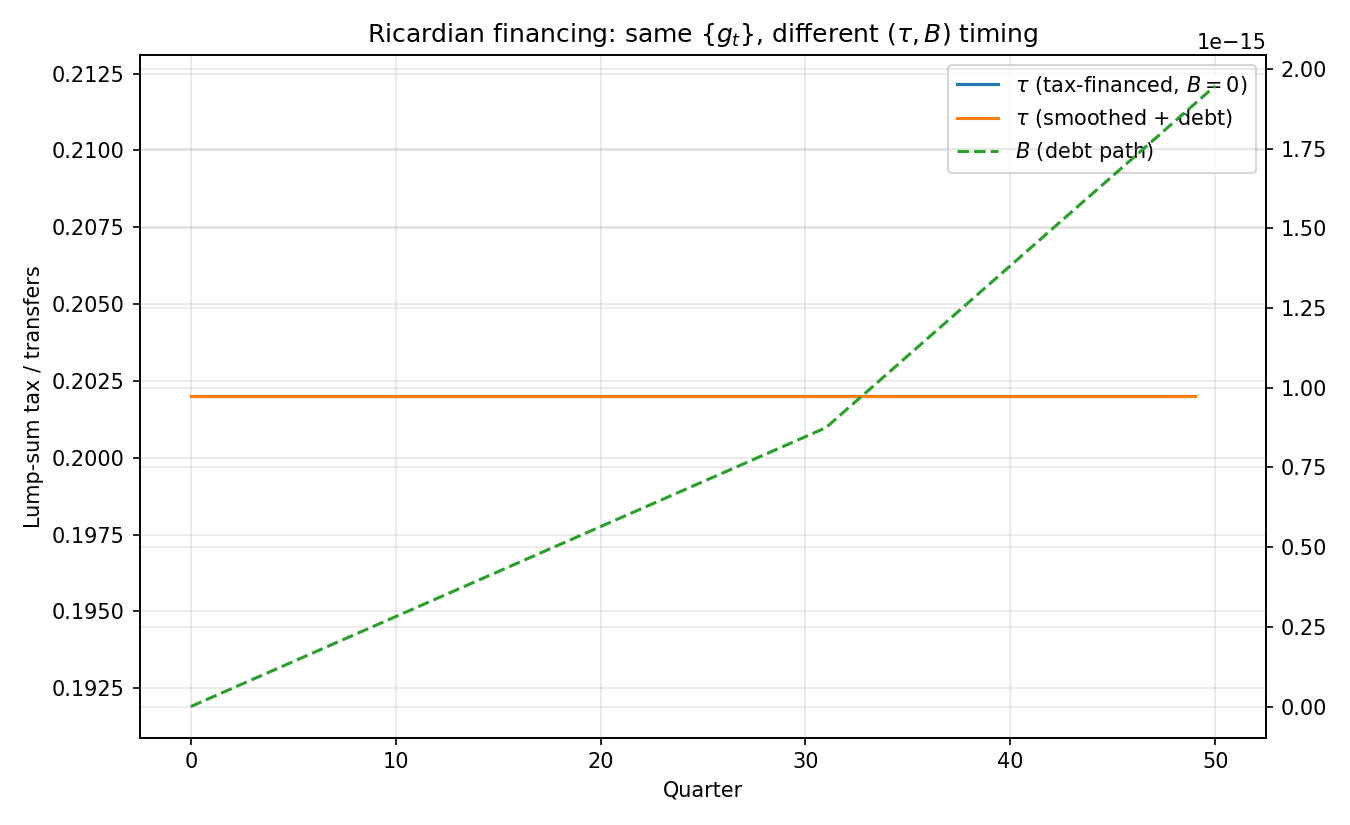
\includegraphics[width=0.92\textwidth]{ricardian_financing.png}
  \caption{Same $\{g_t\}$; alternative $(\tau,B)$ satisfying the flow budget with $q_t$ from the stochastic Euler (not assumed equal to $\beta$).}
  \label{fig:ricardian}
\end{figure}

\paragraph{Breakdown.}
Distortionary labor-income tax financing breaks neutrality; Figure~\ref{fig:breakdown} compares steady states. Dynamic overlays (Figures~\ref{fig:fin_c}--\ref{fig:fin_n}) use an auxiliary perfect-foresight transition calculation for the labor-tax extension.

\begin{figure}[htbp]
  \centering
  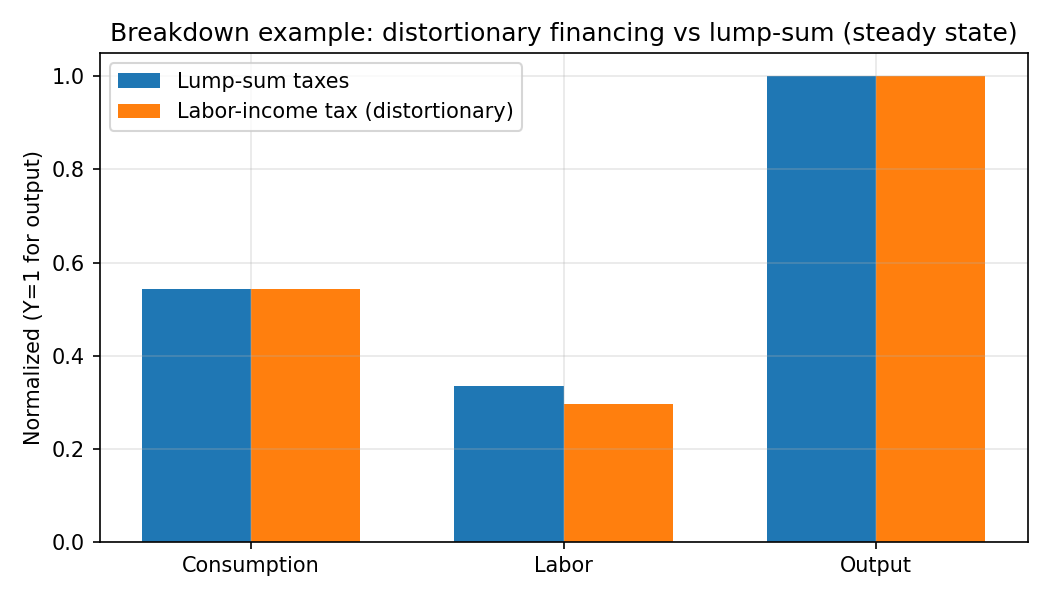
\includegraphics[width=0.65\textwidth]{breakdown_labor_tax_steady_state.png}
  \caption{Steady-state comparison: lump-sum vs.\ distortionary labor tax at the same $g/Y$.}
  \label{fig:breakdown}
\end{figure}

\section{Fiscal spending experiments}

We report three experiments at the productivity state closest to $\bar z$ (tie: $z_L$). The one-time level shock uses $\Delta g = 0.05\,g_{\mathrm{ss}}(\bar z)$ (absolute), the same increment used for $z_L$ vs.\ $z_H$ comparisons and for the foreseen realization at $H=8$. Permanent shift: $+2$ percentage points to $g/y$. Figures~\ref{fig:irf_y}--\ref{fig:irf_i} plot Monte Carlo mean responses ($1200$ draws); Appendix Table~\ref{tab:auto_shock_irf_diag} records the same-run shock normalization and state-dependence summary.

\IfFileExists{../output/report_table_irf_impact_auto.tex}{
  \input{../output/report_table_irf_impact_auto.tex}
}{
  \begin{table}[htbp]
    \centering
    \caption{Unforeseen one-time $g$ shock at $\bar z$ neighborhood: IRF summary ($100\times\log$ ratio, MC mean).}
    \label{tab:irf_impact}
    \begin{tabular}{@{}rcccc@{}}
      \toprule
      Horizon $h$ & $Y$ & $C$ & $N$ & $I$ \\
      \midrule
      $0$ & $4.752$ & $-5.077$ & $7.424$ & $29.875$ \\
      $1$ & $0.177$ & $0.269$ & $-0.210$ & $-0.117$ \\
      $4$ & $0.136$ & $0.266$ & $-0.229$ & $-0.280$ \\
      $8$ & $0.104$ & $0.242$ & $-0.220$ & $-0.340$ \\
      \bottomrule
    \end{tabular}
    \medskip

    \raggedright\small
    \textit{Note:} These are log-percentage IRFs, $100\times \log(x_t^{\text{shock}}/x_t^{\text{base}})$, not fiscal multipliers. The same-run shock normalization appears in Appendix Table~\ref{tab:auto_shock_irf_diag}.
  \end{table}
}

\paragraph{Unforeseen one-time shock.}
On impact, higher $g$ raises output and hours; consumption falls and investment rises in this calibration (Table~\ref{tab:irf_impact}), consistent with a wealth effect and the resource constraint at the stochastic fixed point. The impact percentages look large because the figure and table give each variable's own log-percentage response, not output multipliers: in the baseline replication, the common one-time shock is about $1.0\%$ of baseline output but about $3.9\%$ of baseline investment (Appendix Table~\ref{tab:auto_shock_irf_diag}), so the investment spike is mechanically amplified by a small denominator. In levels at impact, $\Delta y\approx 0.049$, $\Delta c\approx -0.030$, $\Delta i\approx 0.067$, for $\Delta g\approx 0.0124$, i.e.\ an output response about $3.96$ times the spending increment. Figure~\ref{fig:irf_zoom} removes the impact quarter and shows that the post-impact dynamics are smooth and modest rather than numerically erratic.

\paragraph{Foreseen one-time shock.}
The foreseen experiment highlights the genuinely forward-looking side of the model. Because agents internalize the future realization date $H=8$, Figure~\ref{fig:irf_c} shows deviations before the spending increase is actually implemented. That anticipation effect matters because it demonstrates that the model is not merely producing static comparative statics with a Markov label; expectations about future policy move current allocations.

\paragraph{Permanent shift in government size.}
Under the permanent higher-$g/y$ policy, the solved high-spending fixed point features persistently higher hours and output and, in this calibration, slightly \emph{higher} capital rather than lower long-run capital. We therefore do not treat long-run capital crowding out as a generic implication; the pattern is what this solved calibration delivers.

\begin{figure}[htbp]
  \centering
  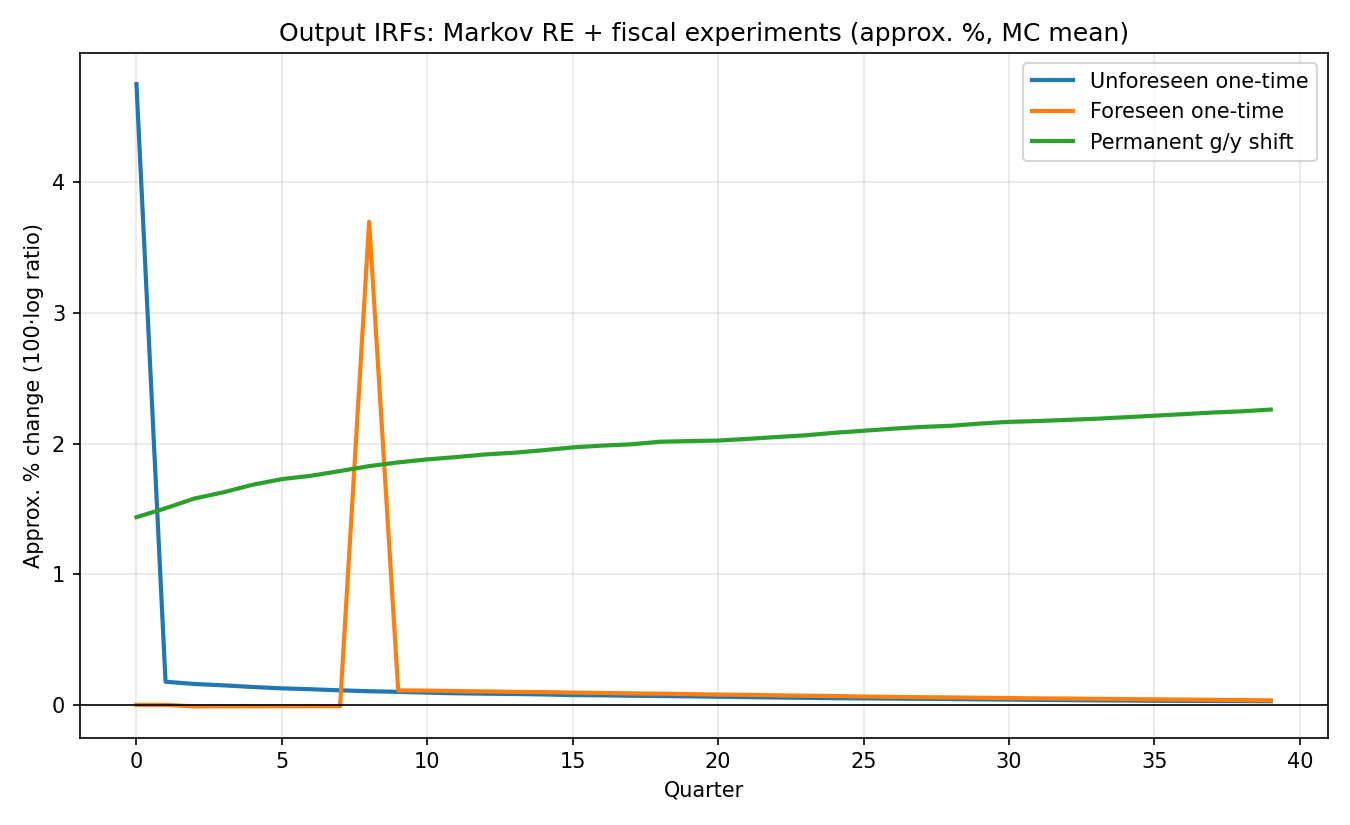
\includegraphics[width=0.92\textwidth]{irf_output_compare.png}
  \caption{Output IRFs (Markov RE, MC mean).}
  \label{fig:irf_y}
\end{figure}
\begin{figure}[htbp]
  \centering
  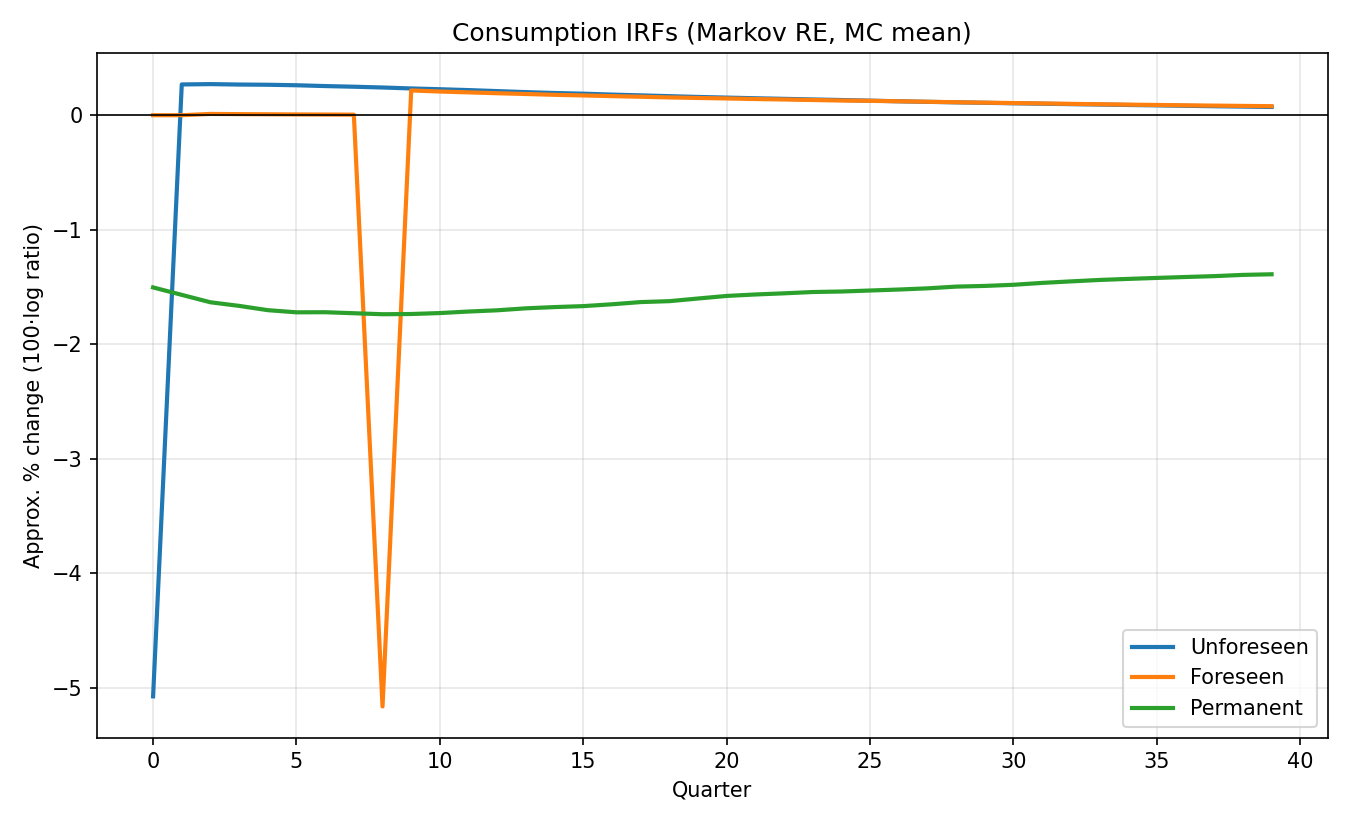
\includegraphics[width=0.92\textwidth]{irf_consumption_compare.png}
  \caption{Consumption IRFs.}
  \label{fig:irf_c}
\end{figure}
\begin{figure}[htbp]
  \centering
  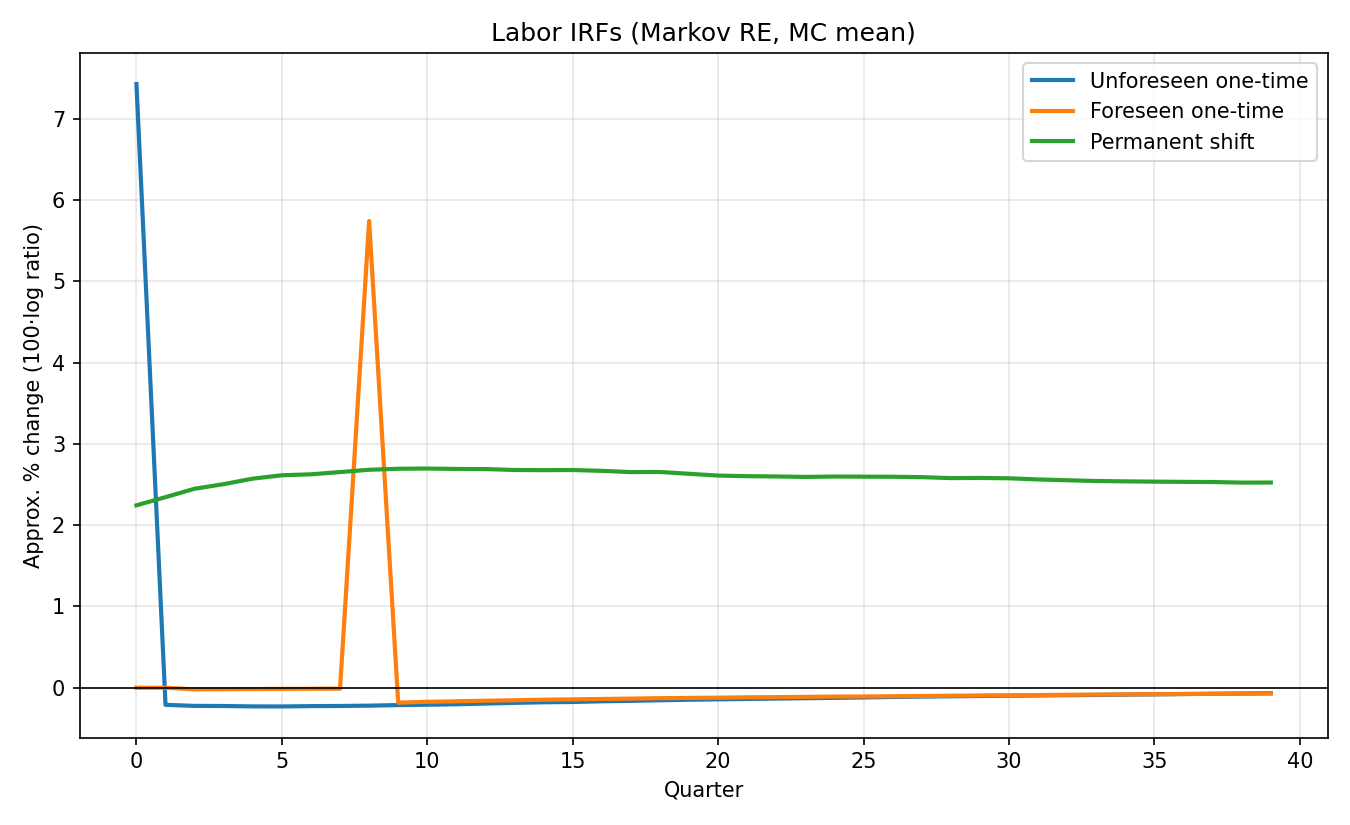
\includegraphics[width=0.92\textwidth]{irf_labor_compare.png}
  \caption{Labor IRFs.}
  \label{fig:irf_n}
\end{figure}
\begin{figure}[htbp]
  \centering
  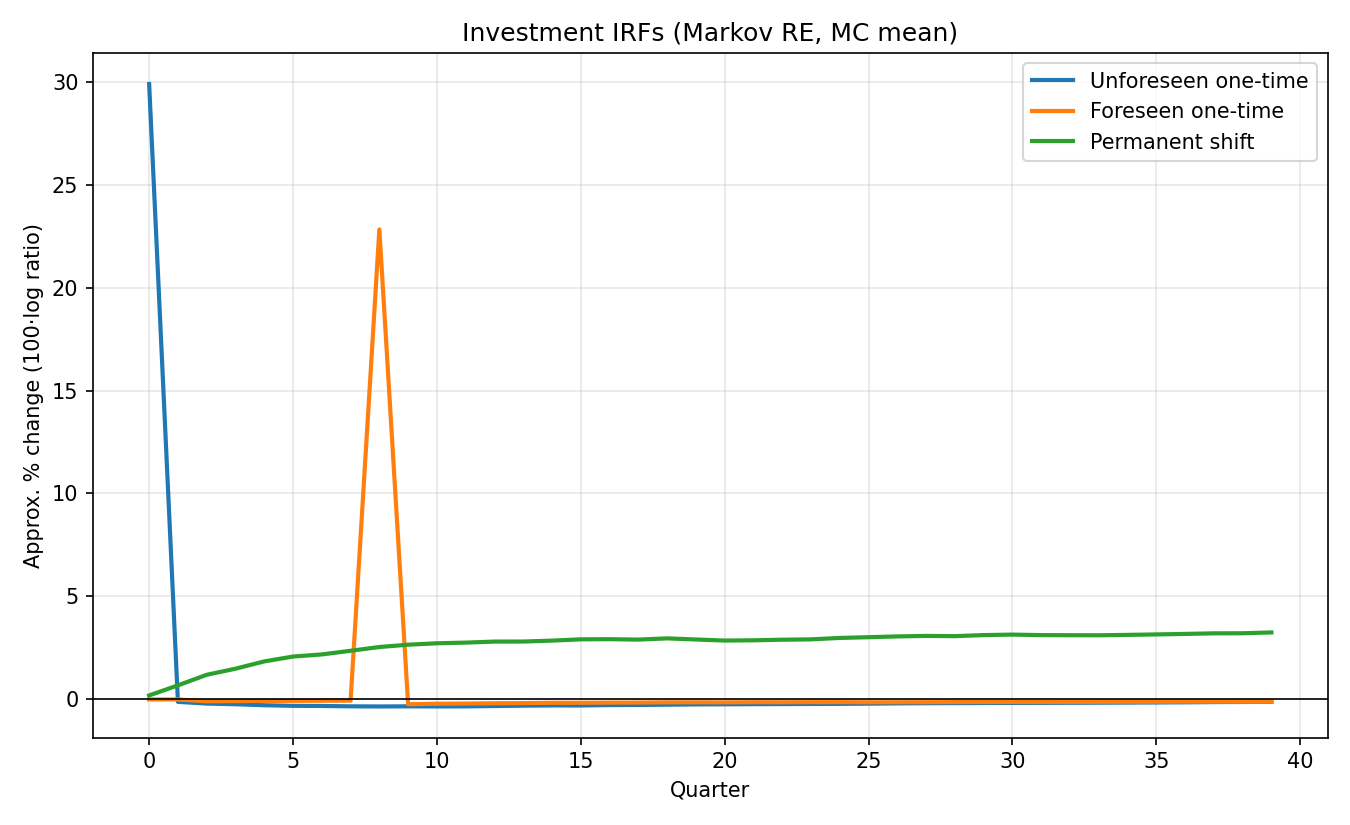
\includegraphics[width=0.92\textwidth]{irf_investment_compare.png}
  \caption{Investment IRFs.}
  \label{fig:irf_i}
\end{figure}
\begin{figure}[htbp]
  \centering
  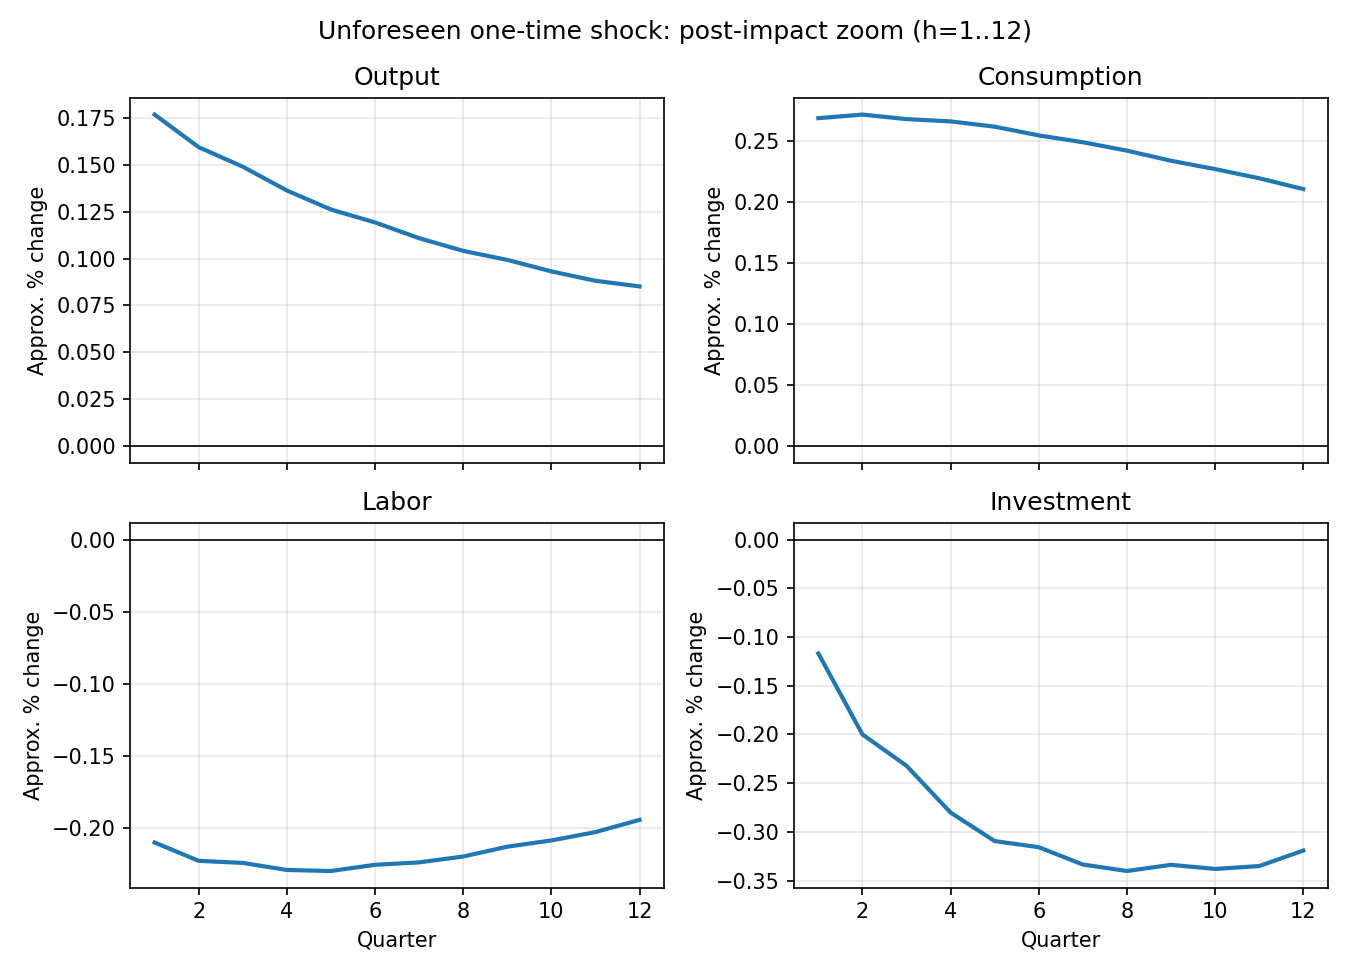
\includegraphics[width=0.92\textwidth]{irf_unforeseen_zoom_h1_12.png}
  \caption{Unforeseen one-time shock: post-impact zoom over horizons $h=1,\dots,12$.}
  \label{fig:irf_zoom}
\end{figure}

\section{Productivity states\texorpdfstring{ ($z_L$ vs.\ $z_H$)}{}}
\label{sec:states}

We initialize at the Markov fixed-point capital for each $z$ (Table~\ref{tab:markov_fp}) and apply the \textbf{same absolute} $\Delta g$ as in Section~6 (from $g_{\mathrm{ss}}(\bar z)$), with MC mean $1200$ draws. Figures~\ref{fig:states_y}--\ref{fig:states_i} contrast responses. At $h=0$, the $z_H-z_L$ gaps are reported in Appendix Table~\ref{tab:auto_shock_irf_diag}; investment retains the largest spread.

The baseline narrow productivity band therefore produces \emph{measured but not explosive} state dependence: at impact, $z_H-z_L$ equals $0.53$ log points for output, $-0.54$ for consumption, $0.82$ for labor, and $4.12$ for investment. In the high-productivity state, the same absolute spending increase can be accommodated with less immediate consumption sacrifice and a stronger investment response because marginal products are higher. A wider productivity spread $z_L=0.90$, $z_H=1.10$ (re-solved value function, MC mean with $800$ draws per state) is reported in Figure~\ref{fig:states_wide} as a sensitivity check on state dependence.

\begin{figure}[htbp]
  \centering
  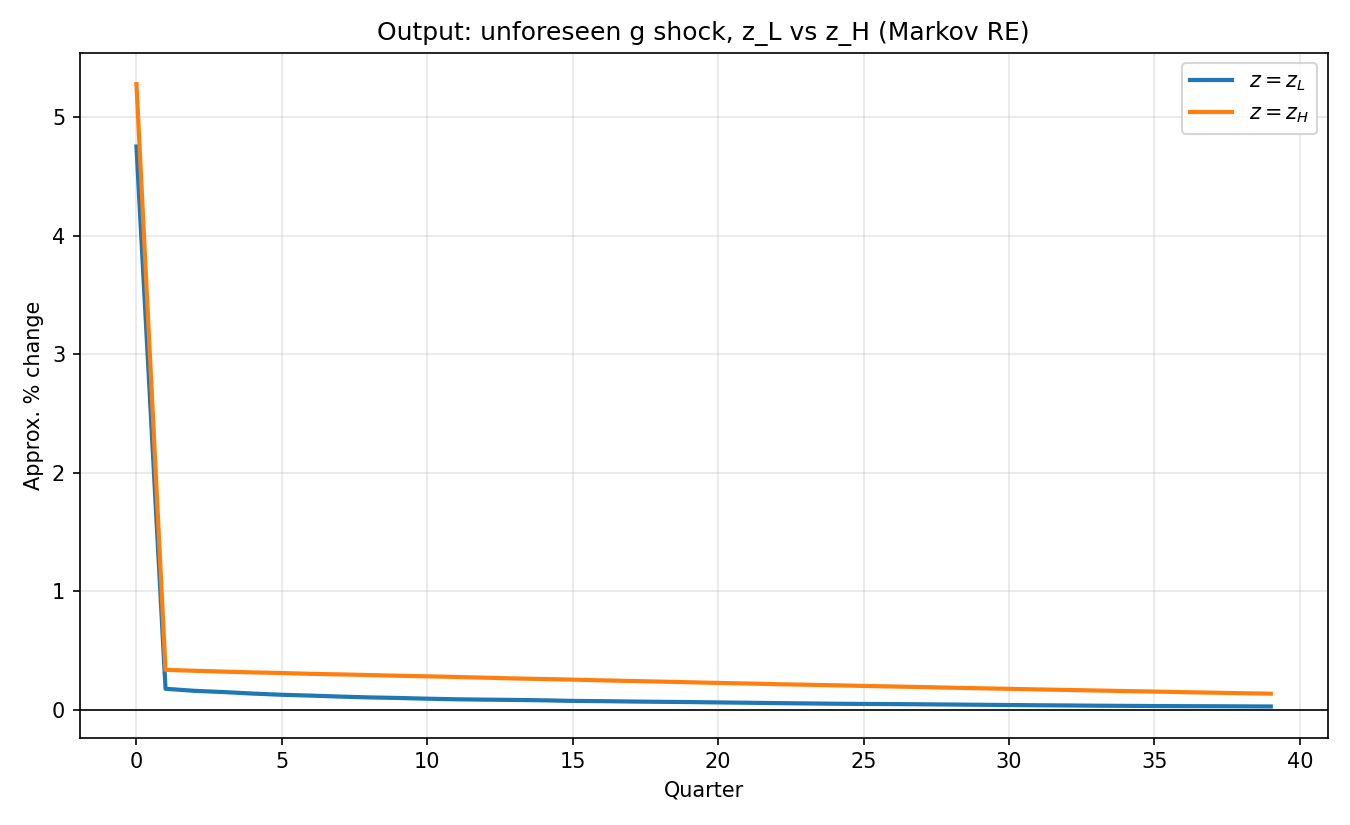
\includegraphics[width=0.92\textwidth]{irf_output_zL_zH.png}
  \caption{Output: $z_L$ vs.\ $z_H$.}
  \label{fig:states_y}
\end{figure}
\begin{figure}[htbp]
  \centering
  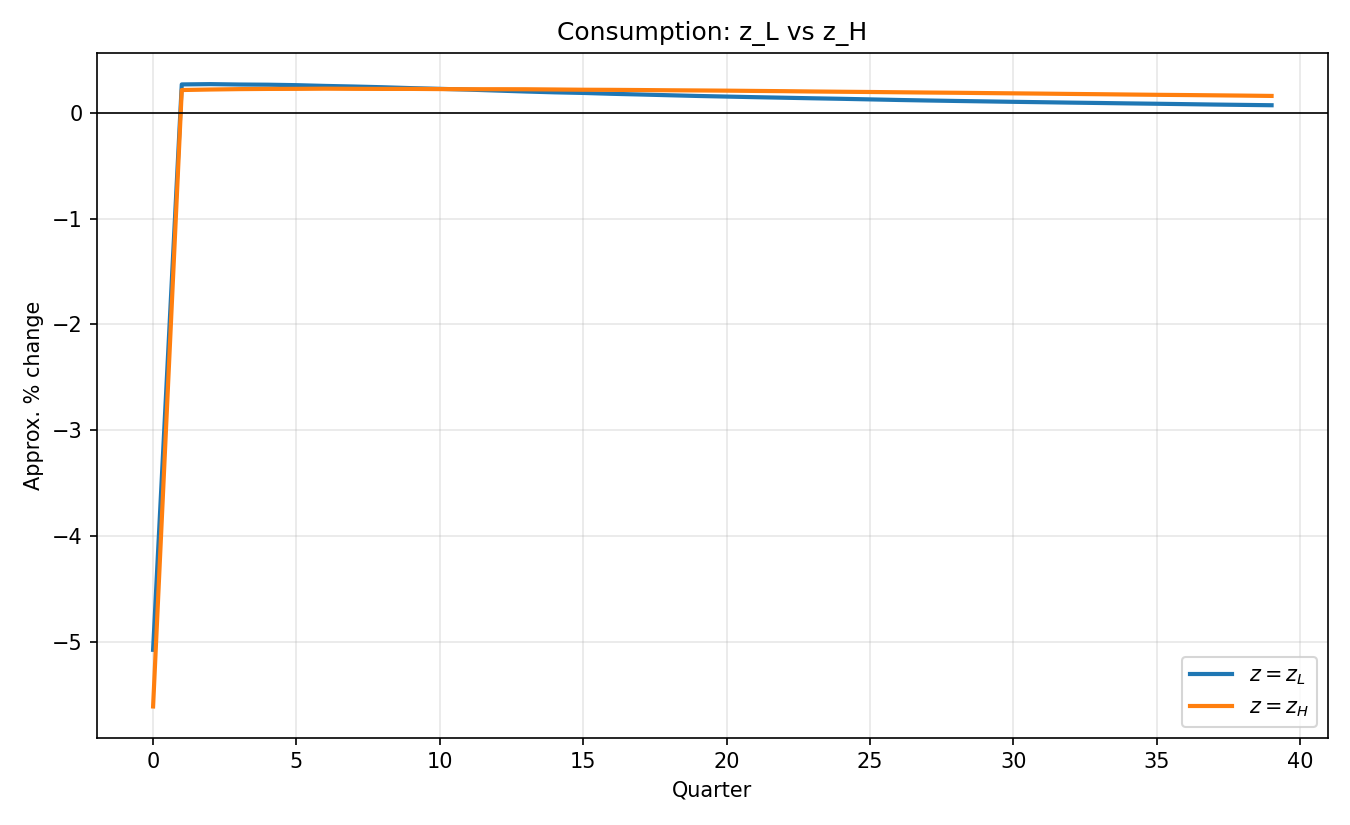
\includegraphics[width=0.92\textwidth]{irf_consumption_zL_zH.png}
  \caption{Consumption: $z_L$ vs.\ $z_H$.}
  \label{fig:states_c}
\end{figure}
\begin{figure}[htbp]
  \centering
  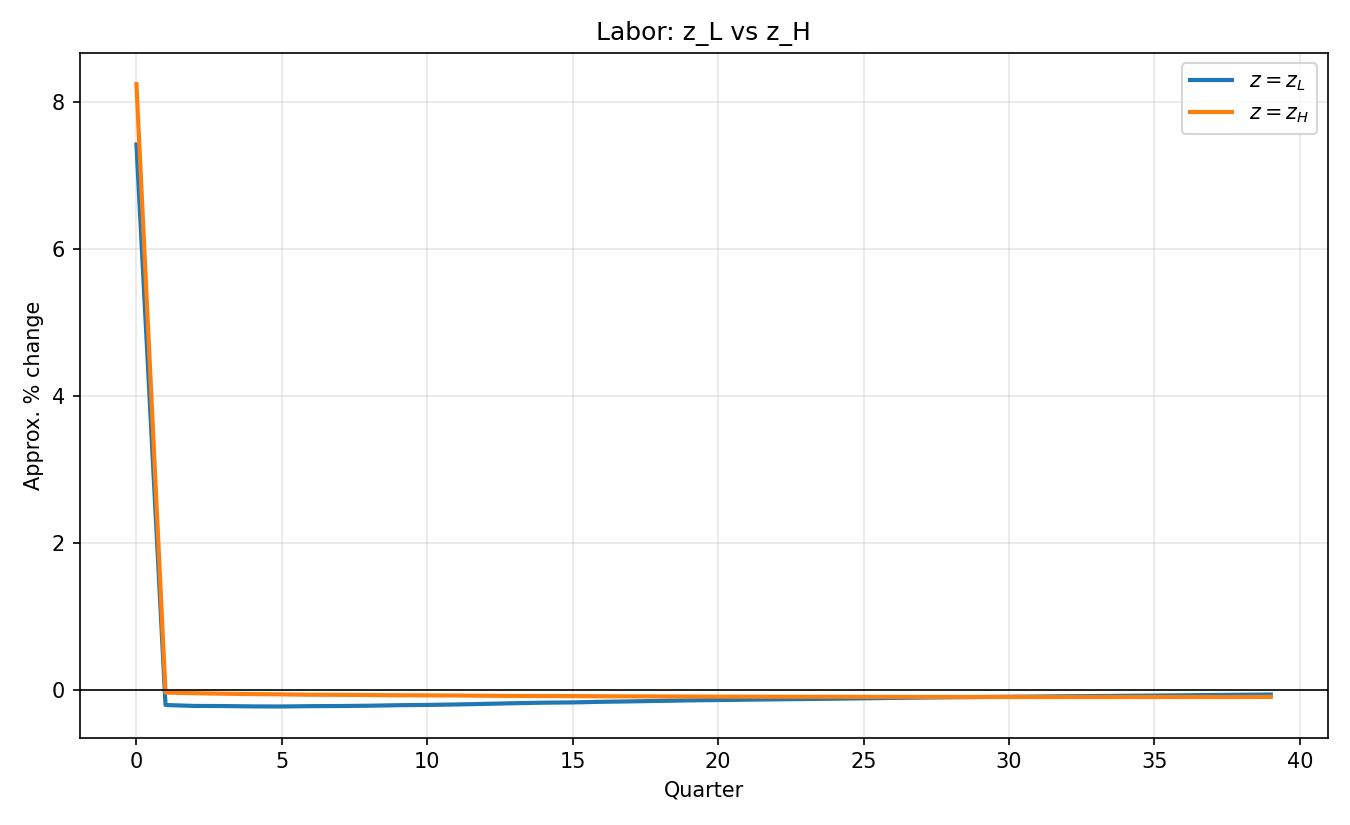
\includegraphics[width=0.92\textwidth]{irf_labor_zL_zH.png}
  \caption{Labor: $z_L$ vs.\ $z_H$.}
  \label{fig:states_n}
\end{figure}
\begin{figure}[htbp]
  \centering
  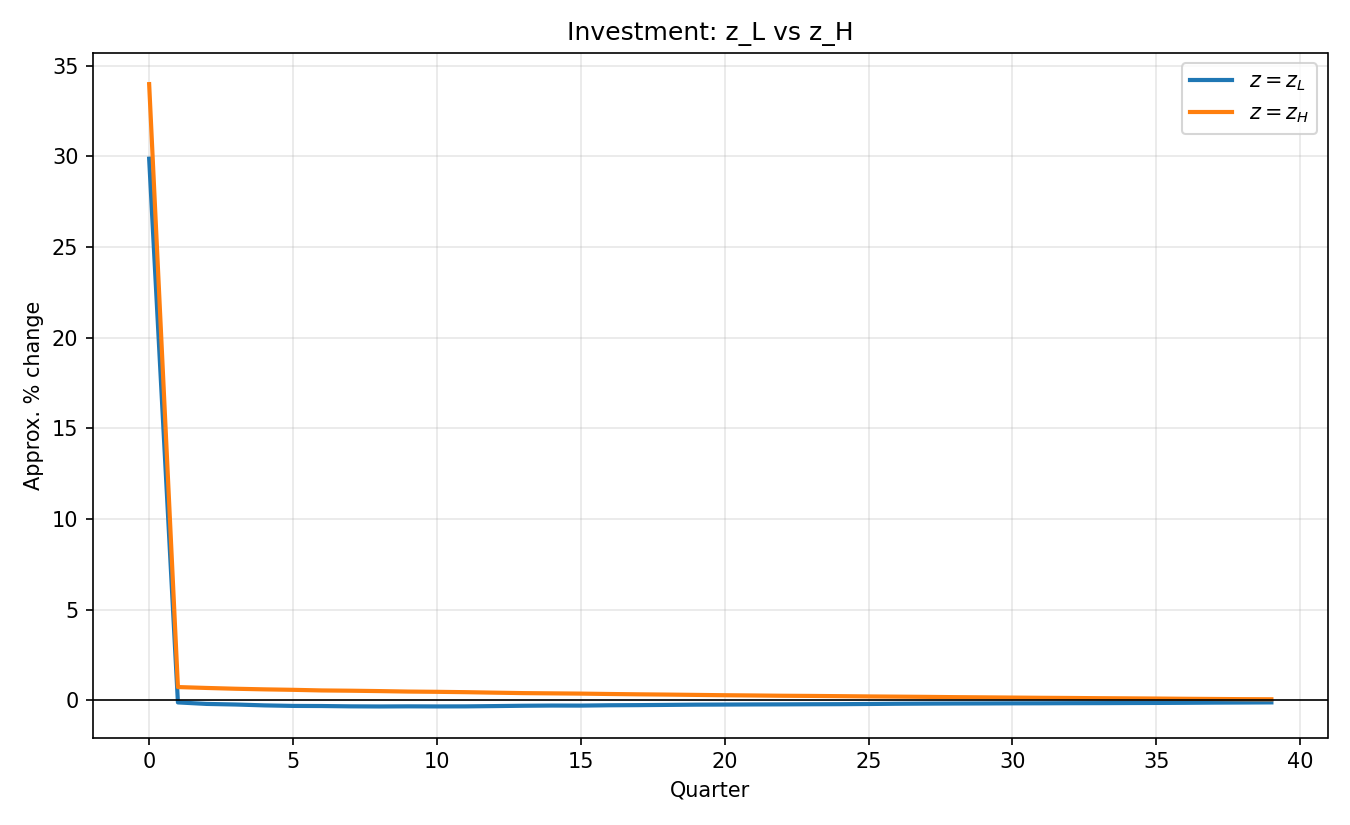
\includegraphics[width=0.92\textwidth]{irf_investment_zL_zH.png}
  \caption{Investment: $z_L$ vs.\ $z_H$.}
  \label{fig:states_i}
\end{figure}

\begin{figure}[htbp]
  \centering
  \begin{subfigure}[b]{0.48\textwidth}
    \centering
    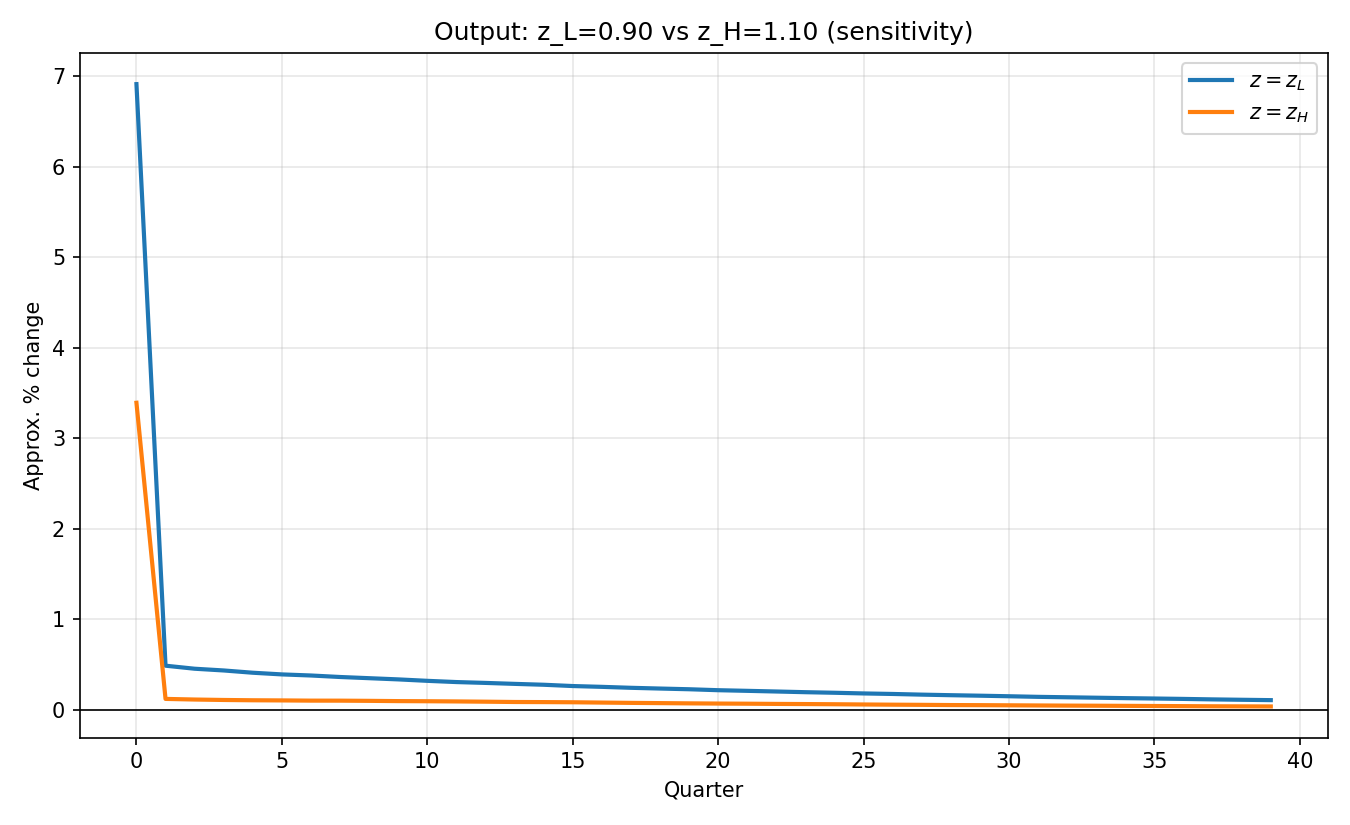
\includegraphics[width=\textwidth]{irf_output_zL_zH_wide.png}
    \caption{Output.}
  \end{subfigure}
  \hfill
  \begin{subfigure}[b]{0.48\textwidth}
    \centering
    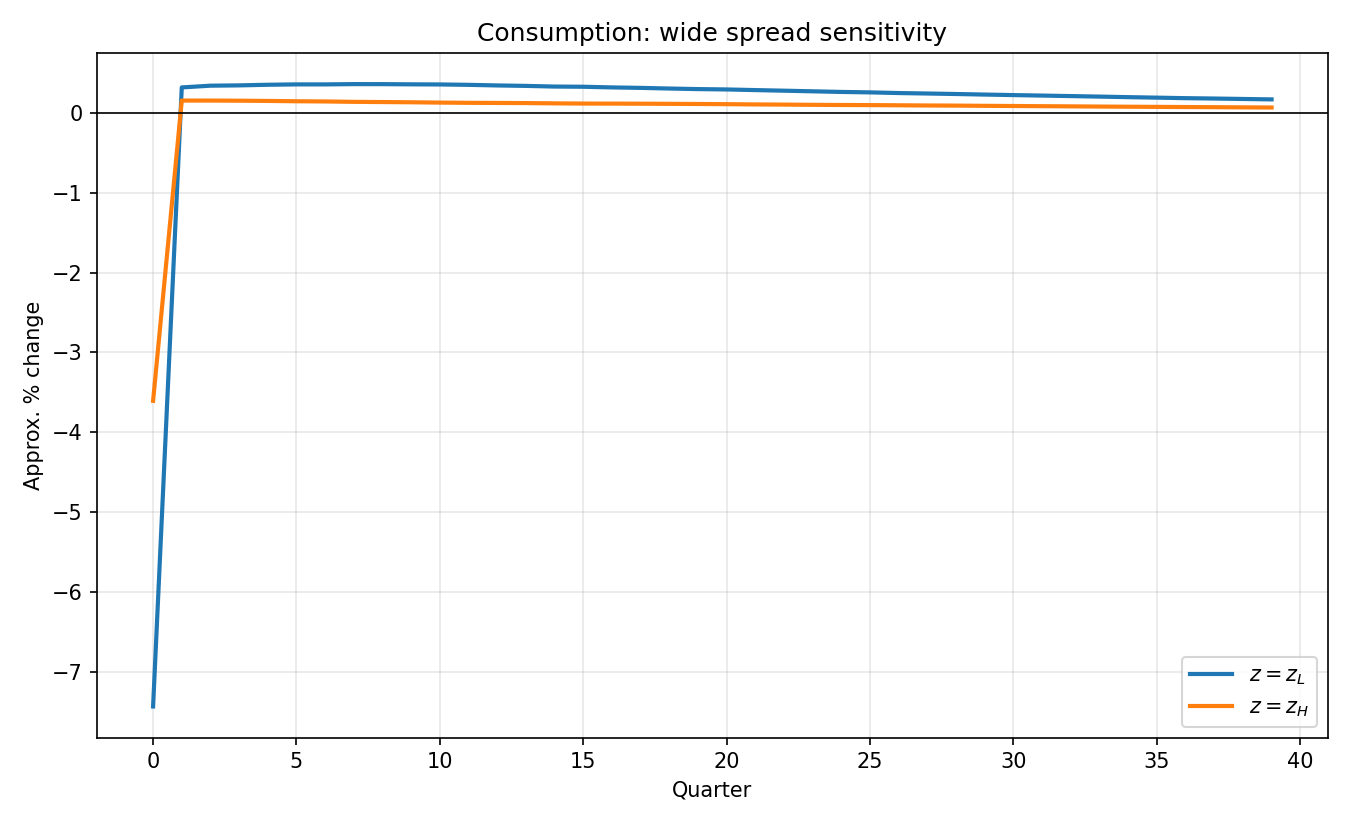
\includegraphics[width=\textwidth]{irf_consumption_zL_zH_wide.png}
    \caption{Consumption.}
  \end{subfigure}
  \vspace{0.6em}
  \begin{subfigure}[b]{0.48\textwidth}
    \centering
    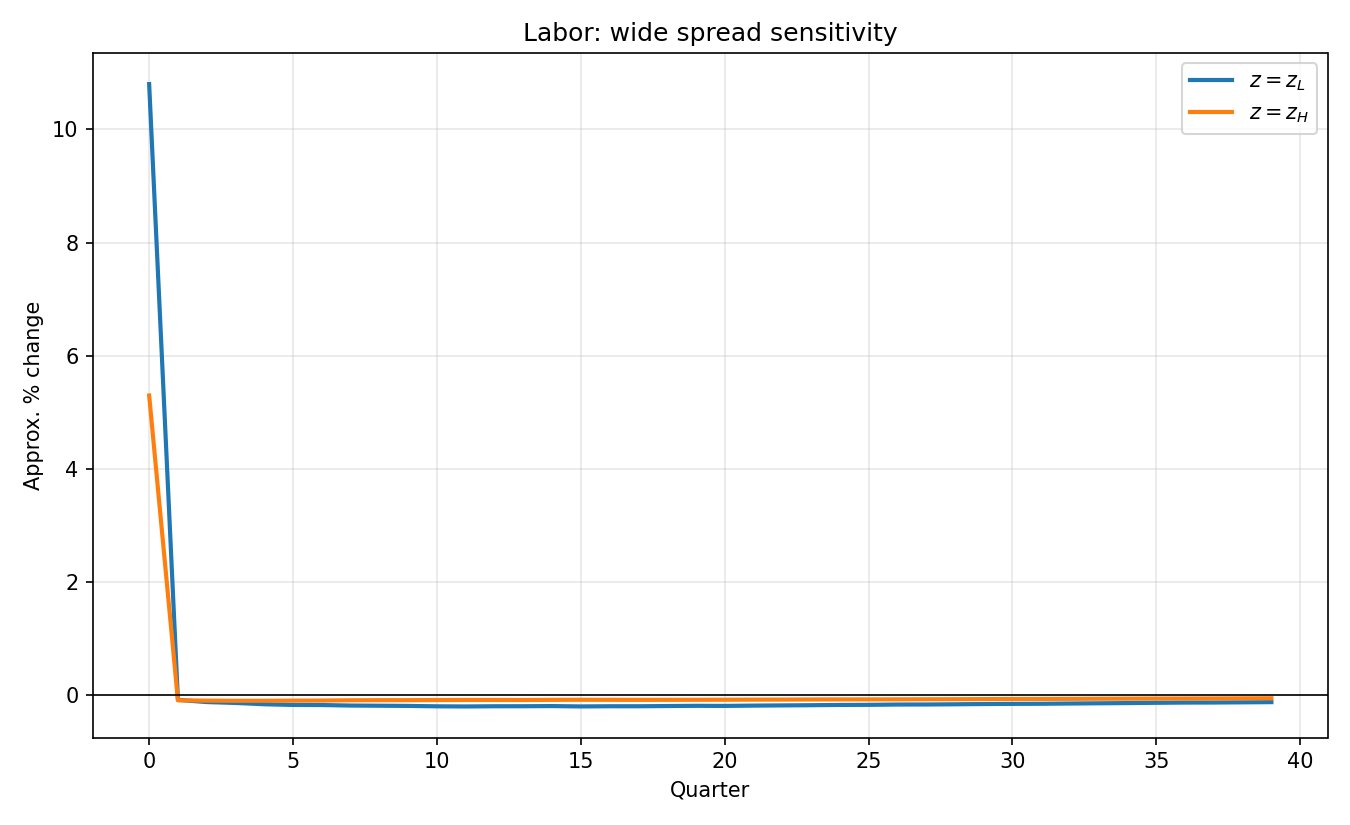
\includegraphics[width=\textwidth]{irf_labor_zL_zH_wide.png}
    \caption{Labor.}
  \end{subfigure}
  \hfill
  \begin{subfigure}[b]{0.48\textwidth}
    \centering
    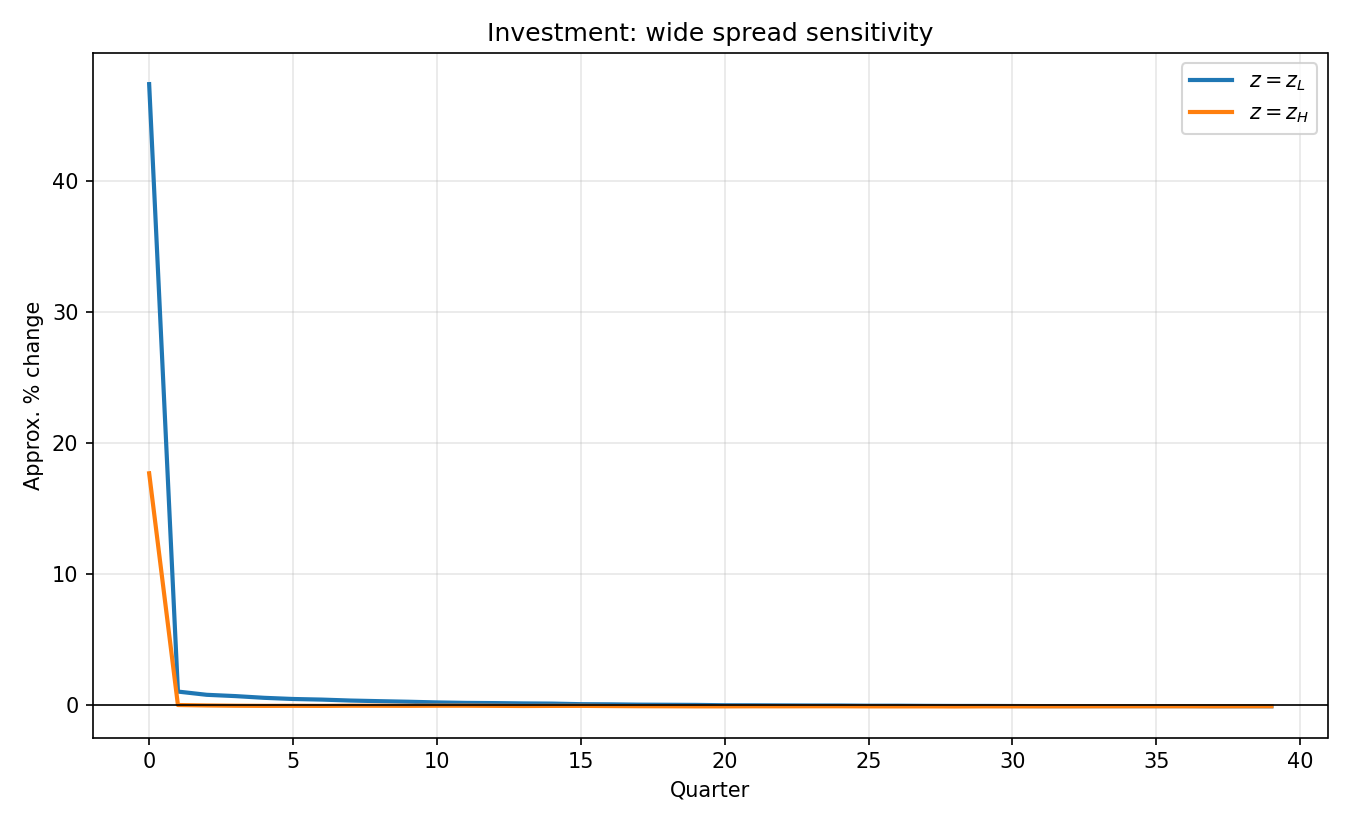
\includegraphics[width=\textwidth]{irf_investment_zL_zH_wide.png}
    \caption{Investment.}
  \end{subfigure}
  \caption{Wider productivity spread (sensitivity).}
  \label{fig:states_wide}
\end{figure}

\section{Comparison with empirical evidence}
\label{sec:empirical}

We combine own empirical work with a literature-led comparison. Quarterly U.S.\ macro series from FRED (real GDP, consumption, investment, government consumption, hours) are transformed as $100\times\Delta\log(\cdot)$ to approximate quarterly percent changes. Sample coverage and data construction are summarized in Appendix Table~\ref{tab:auto_emp_diag}. All empirical numbers use a \emph{fixed} quarterly dataset (1980Q1--2025Q4: $184$ observations in levels, $183$ in transformed growth rates), held constant across replications so results are not sensitive to post-sample revisions or downloads.

\paragraph{Reduced-form VAR.}
We estimate a VAR(4) in $(G,Y,C,I,H)$ with baseline Cholesky ordering $G\to Y\to C\to I\to H$ and plot orthogonalized impulse responses to a one-standard-deviation innovation to $G$. Table~\ref{tab:var_impact} records the contemporaneous responses from the same frozen-data run as Figure~\ref{fig:emp_var}; Appendix Table~\ref{tab:auto_emp_diag} reports the corresponding sample diagnostics. In this replication, the innovation raises $G$ by $0.733$ on impact but moves $Y$, $C$, $I$, and $H$ by $-0.088$, $-0.187$, $-0.683$, and $-0.341$, respectively. That sign pattern contrasts sharply with the model's impact responses for output and hours. These designs are \emph{not} narrative military spending shocks; they provide transparent reduced-form moments to juxtapose with the model.

\IfFileExists{../output/report_table_var_impact_auto.tex}{
  \input{../output/report_table_var_impact_auto.tex}
}{
  \begin{table}[htbp]
    \centering
    \caption{Data VAR: impact responses to a one s.d.\ orthogonalized $G$ innovation (baseline Cholesky $G,Y,C,I,H$).}
    \label{tab:var_impact}
    \begin{tabular}{@{}lrrrrr@{}}
      \toprule
      $h=0$ & $G$ & $Y$ & $C$ & $I$ & $H$ \\
      \midrule
      Response & $0.484$ & $0.154$ & $-0.141$ & $0.599$ & $-0.074$ \\
      \bottomrule
    \end{tabular}
    \medskip

    \raggedright\small
    \textit{Note:} Units match the transformed data (approximate quarterly percentage change). The frozen-data sample and first-stage diagnostics are reported in Appendix Table~\ref{tab:auto_emp_diag}.
  \end{table}
}

\paragraph{Local projections.}
Figure~\ref{fig:emp_lp} reports HAC local-projection IRFs using the first-equation VAR residual under the recursive baseline order as the fiscal innovation. Horizon-by-horizon estimation relaxes the restriction that all dynamics are summarized by a single VAR transition matrix, providing a robustness check on the model--data comparison.

\paragraph{IV local projections.}
Figure~\ref{fig:emp_iv} reports \textbf{two-stage} local projections: $\Delta\log G_t$ is instrumented by its value two quarters earlier (predetermined in the $\Delta\log$ panel), with four lags of $(G,Y,C,I,H)$ as controls; second-stage HAC standard errors. This is \emph{not} narrative identification (contrast \citet{ramey2011identifying}); first-stage strength is reported in Appendix Table~\ref{tab:auto_emp_diag}. In the baseline frozen-data replication, the horizon-$0$ first-stage statistic is only $2.1307$, so the IV-LP results are a weak-instrument robustness exercise rather than a decisively identified estimate.

\paragraph{Impact scorecard.}
Table~\ref{tab:model_data_impact} places the benchmark model beside the three empirical estimators from the same replication as the figures and appendix diagnostics. The recursive VAR and VAR-residual LP agree on negative impact responses for output, consumption, investment, and hours, whereas the model predicts positive output, labor, and investment together with negative consumption. IV-LP narrows the gap by turning output, consumption, and hours positive on impact, but the weak first stage precludes treating that row as validation of the model.

\IfFileExists{../output/report_table_model_data_impact_auto.tex}{
  \input{../output/report_table_model_data_impact_auto.tex}
}{
  \begin{table}[htbp]
    \centering
    \caption{Impact responses: model and data side by side (native units).}
    \label{tab:model_data_impact}
    \small
    \begin{tabular}{@{}lrrrr@{}}
      \toprule
      Specification & $Y$ & $C$ & $I$ & $N/H$ \\
      \midrule
      Model: Markov RBC, unforeseen one-time $g$ shock & $4.752$ & $-5.077$ & $29.875$ & $7.424$ \\
      Data: recursive VAR & $-0.088$ & $-0.187$ & $-0.683$ & $-0.341$ \\
      Data: VAR-residual LP & $-0.120$ & $-0.255$ & $-0.932$ & $-0.465$ \\
      Data: IV-LP & $0.352$ & $0.347$ & $-0.142$ & $0.251$ \\
      \bottomrule
    \end{tabular}
    \medskip

    \raggedright\small
    \textit{Note:} The model row reports $100\times\log(x_t^{\mathrm{shock}}/x_t^{\mathrm{base}})$ at $h=0$ for the unforeseen one-time spending shock; empirical rows report impact coefficients from the frozen-sample VAR, VAR-residual local projections, and IV local projections. The model uses labor $N$, while empirical rows use hours $H$. Scales are therefore not directly comparable; the table is intended for sign and pattern comparison. The IV first-stage statistic at $h=0$ is $2.1307$, so the IV row should be read with the weak-instrument caveat.
  \end{table}
}

\begin{figure}[htbp]
  \centering
  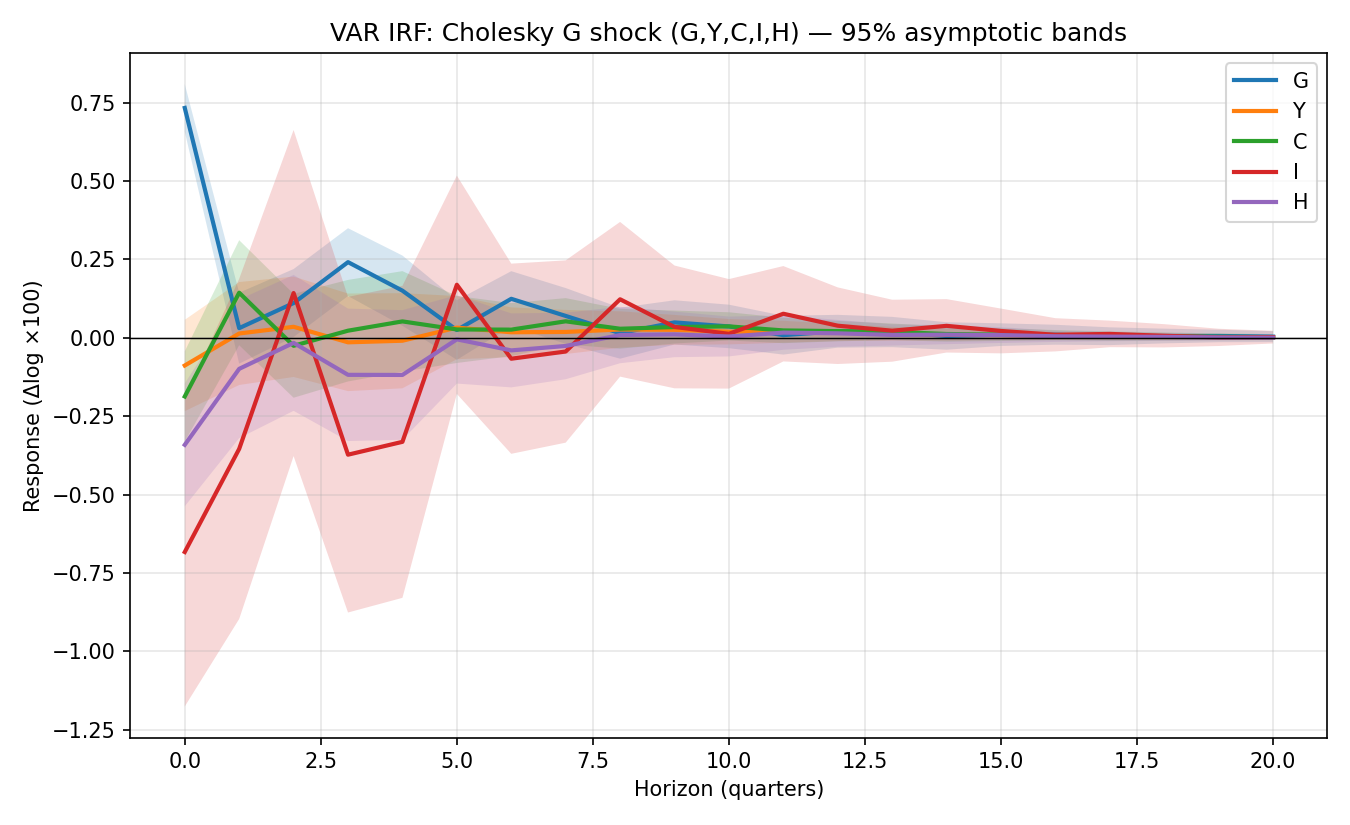
\includegraphics[width=0.92\textwidth]{empirical_var_irf_g_shock.png}
  \caption{Data: VAR IRFs (Cholesky; shock to ordering position of $G$). Sample and ordering diagnostics are summarized in Appendix Table~\ref{tab:auto_emp_diag}.}
  \label{fig:emp_var}
\end{figure}
\begin{figure}[htbp]
  \centering
  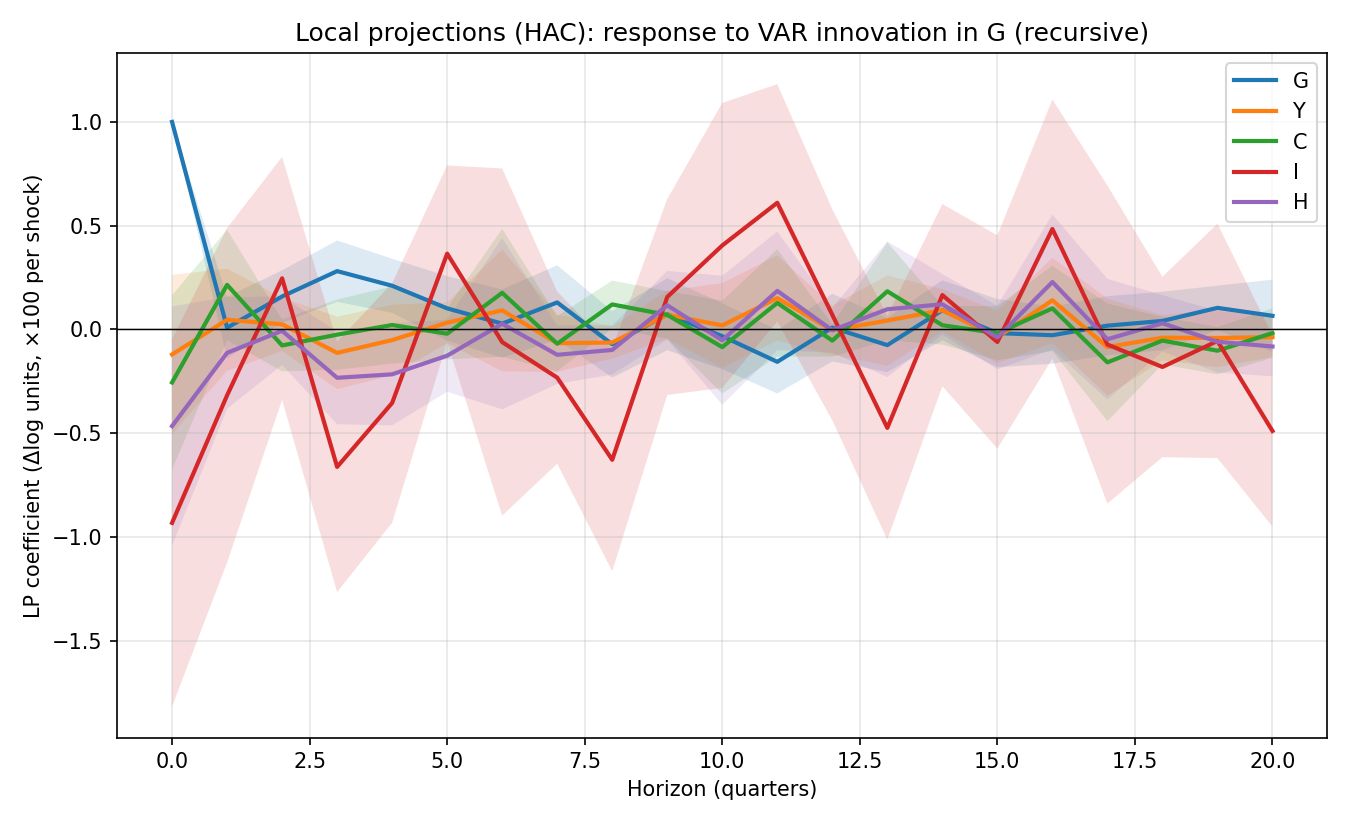
\includegraphics[width=0.92\textwidth]{empirical_local_projection.png}
  \caption{Local-projection responses to the VAR residual fiscal innovation (HAC standard errors).}
  \label{fig:emp_lp}
\end{figure}
\begin{figure}[htbp]
  \centering
  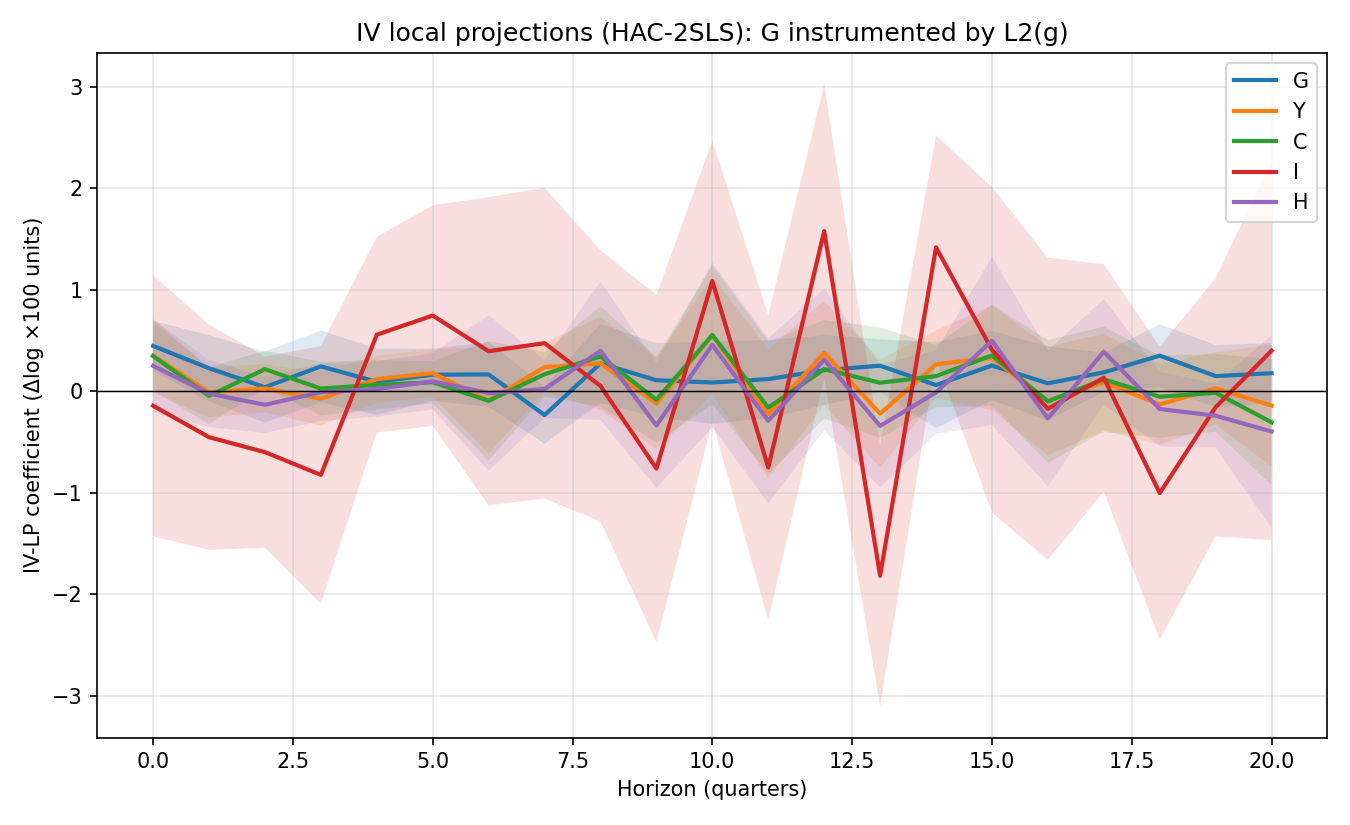
\includegraphics[width=0.92\textwidth]{empirical_iv_lp.png}
  \caption{IV local projections (HAC-2SLS): responses to an instrumented fiscal spending innovation.}
  \label{fig:emp_iv}
\end{figure}

\paragraph{Literature anchors.}
Canonical references (alongside the reduced-form moments above):
\begin{itemize}
  \item \citet{blanchard2002empirical}: institutional timing restrictions in quarterly fiscal VARs; private consumption and investment patterns often richer than the frictionless RBC benchmark.
  \item \citet{ramey2011identifying}: narrative defense news; highlights anticipation and timing distinct from reduced-form ordering assumptions.
  \item \citet{auerbach2012output}: strong \emph{state dependence} of multipliers---recessions vs.\ expansions---beyond what a narrow productivity gap alone generates.
\end{itemize}

\begin{table}[htbp]
  \centering
  \caption{Model vs.\ broad empirical patterns (qualitative).}
  \label{tab:lit}
  \small
  \begin{tabular}{@{}>{\raggedright\arraybackslash}p{2.2cm}>{\raggedright\arraybackslash}p{5.2cm}>{\raggedright\arraybackslash}p{5.0cm}@{}}
    \toprule
    Margin & Stochastic RBC benchmark & VAR/LP moments + identified / narrative evidence \\
    \midrule
    $Y$ & Positive short-run response to higher $g$ & Our recursive VAR/LP are negative on impact; positive responses remain common in other designs and the literature \\
    $C$ & Crowding out on impact, then mild rebound in the one-time shock experiment & Our recursive VAR/LP are also negative on impact; some identified designs turn positive \\
    $N,H$ & Strong impact increase; smaller post-impact one-time responses & Our recursive estimates are negative on impact; hours remain identification-sensitive \\
    $I$ & Large impact spike, mild medium-run crowding out in the one-time shock, positive under permanent higher $g/y$ & Our recursive VAR/LP are negative on impact; investment is especially identification-sensitive \\
    State dep. & Limited for narrow $z_L,z_H$ & Large recession--expansion gaps possible (AG) \\
    \bottomrule
  \end{tabular}
\end{table}

\section{Extension: distortionary financing (auxiliary PF)}

This extension is deliberately separated from the main Markov benchmark. Its role is diagnostic: once government spending is financed by a labor-income tax, the tax wedge enters the intratemporal condition directly, so the timing and composition of financing now matter for real allocations even if the spending path is held fixed. The steady-state comparison in Figure~\ref{fig:breakdown} and the dynamic overlays in Figures~\ref{fig:fin_c}--\ref{fig:fin_n} therefore provide a clean counterexample to Ricardian neutrality under distortionary instruments.

\begin{figure}[htbp]
  \centering
  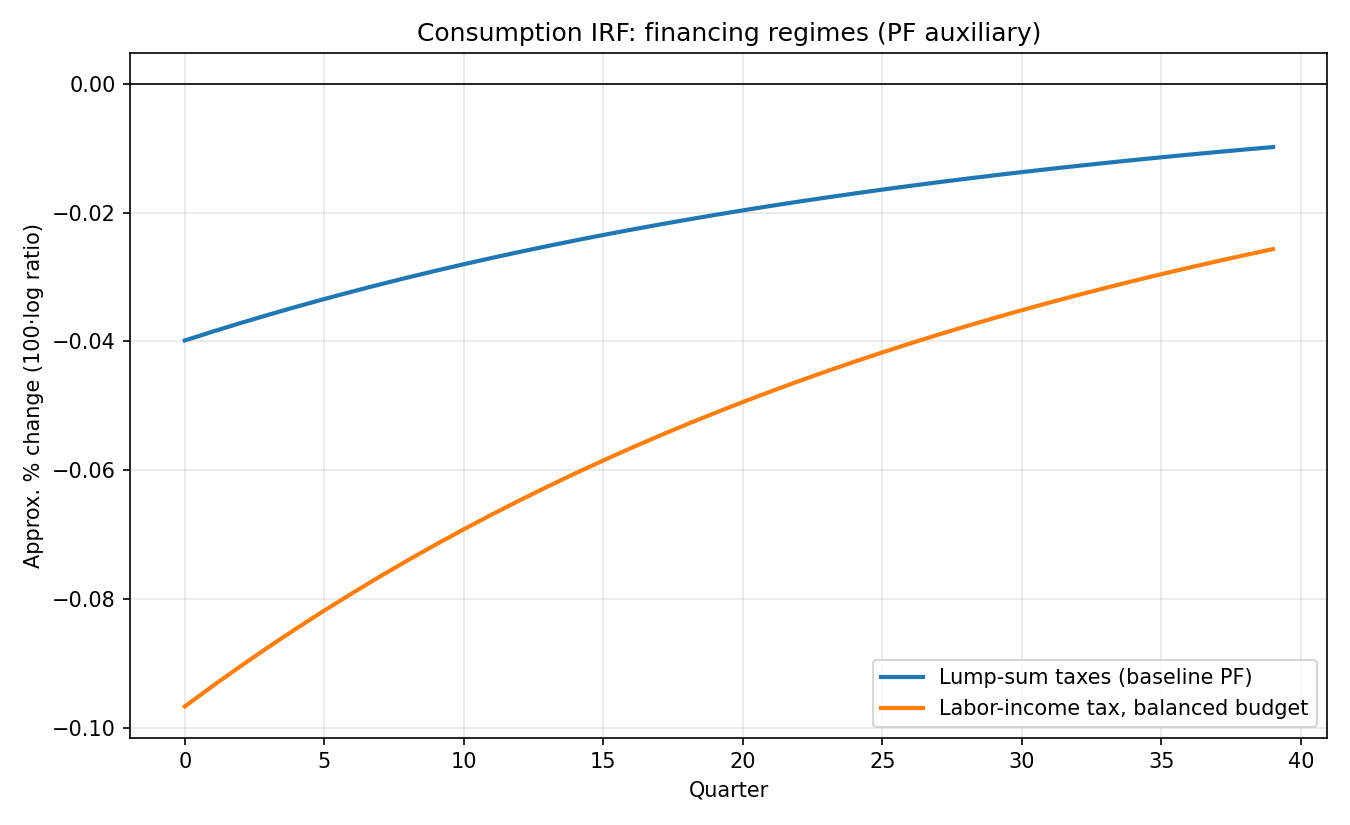
\includegraphics[width=0.92\textwidth]{irf_consumption_financing_regimes.png}
  \caption{Consumption: lump-sum vs.\ labor-tax financing (PF auxiliary).}
  \label{fig:fin_c}
\end{figure}
\begin{figure}[htbp]
  \centering
  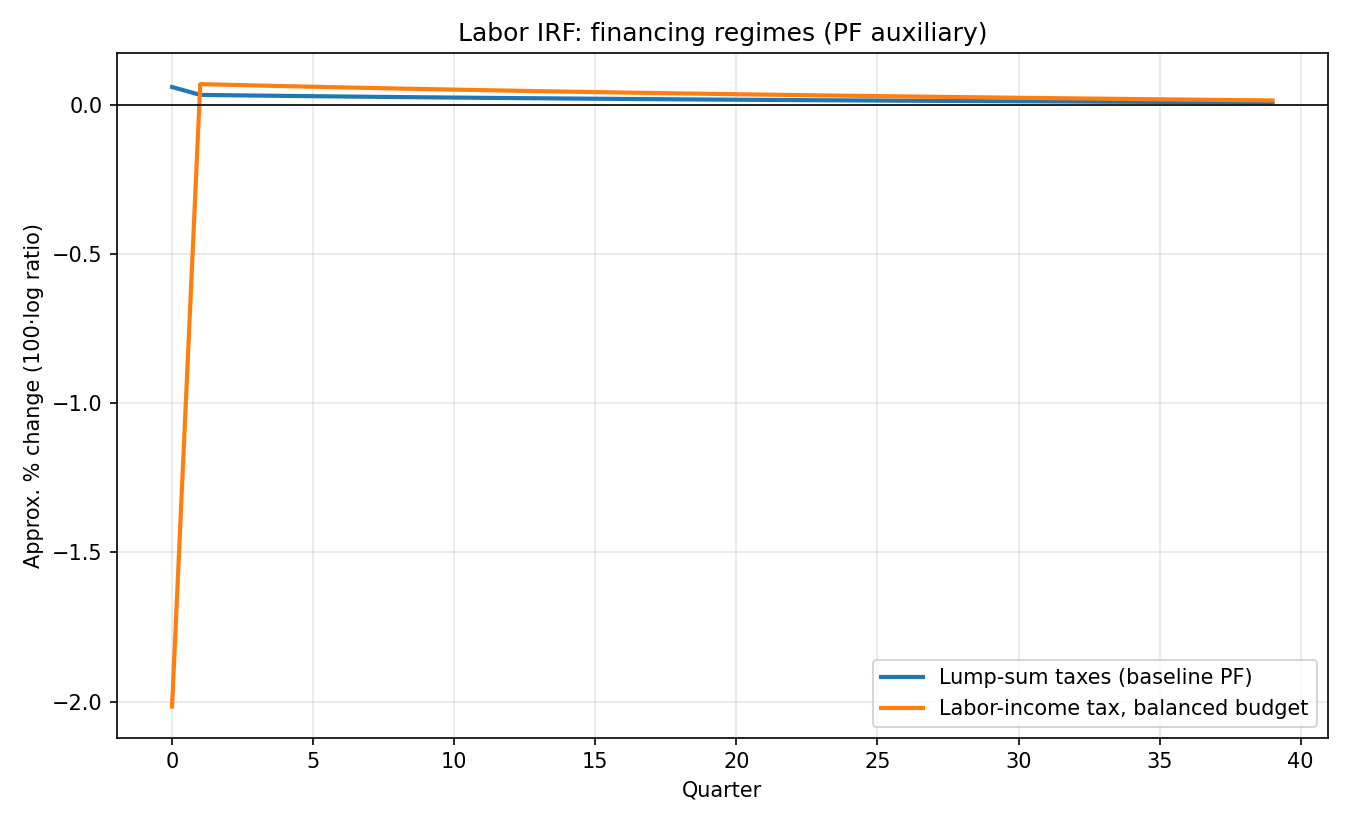
\includegraphics[width=0.92\textwidth]{irf_labor_financing_regimes.png}
  \caption{Labor IRFs under the same comparison.}
  \label{fig:fin_n}
\end{figure}

\section{Interpretation and limitations}

The strongest reading of this paper is as a transparent, internally consistent benchmark, not as a definitive account of fiscal multipliers. Four limitations stand out. First, state dependence enters only through a two-state productivity process, whereas much empirical work emphasizes slack, unemployment, financial constraints, or the zero lower bound. Second, the benchmark omits nominal rigidities and hand-to-mouth households, which are often invoked to rationalize stronger short-run demand and less negative consumption responses. Third, the IV design is deliberately simple and weak, so the empirical block documents sensitivity more than sharp identification. Fourth, some model moments, especially investment IRFs, reflect denominator effects: the spending innovation is modest relative to output but larger relative to baseline investment.

Stating these limits clarifies the contribution: we characterize what the frictionless stochastic RBC benchmark delivers, verify Ricardian logic numerically, and indicate where richer mechanisms would be needed to align with narrative-shock or recession-state evidence.

\section{Conclusion}

The Markov rational-expectations fiscal RBC model delivers a transparent laboratory: lump-sum finance preserves neutrality of debt versus tax timing when bond prices respect the household's stochastic discount factor, while spending shocks move aggregates along paths that integrate uncertainty about future $z$. In the baseline calibration, the common one-quarter spending increase raises output and hours on impact, crowds out consumption, and produces a large percentage investment response because the spending increment is sizable relative to investment's baseline denominator. Ricardian equivalence is not just asserted but numerically verified through zero flow-budget residuals and zero allocation differences across financing regimes at reported precision.

The empirical comparison is sobering. In the fixed quarterly U.S.\ sample (1980Q1--2025Q4), the recursive VAR implies negative impact responses for output, consumption, investment, and hours, while IV-LP is too weakly identified to resolve the discrepancy cleanly. The model aligns most clearly with those recursive moments on impact consumption crowding out, not on output--hours comovement. Relative to narrative identification and recession-state multiplier evidence, the frictionless benchmark remains incomplete. The substantive conclusion is that the model works well as a reproducible laboratory for Ricardian logic and stochastic fiscal propagation, but matching broader fiscal evidence likely requires distortionary finance, hand-to-mouth behavior, nominal rigidities, or richer shock identification.

\appendix
\IfFileExists{../output/report_appendix_auto.tex}{
  \input{../output/report_appendix_auto.tex}
}{
  \section{Appendix (placeholder)}
  Numerical diagnostics are included when the replication pipeline is run; this build uses inline fallback tables where automated inputs are absent.
}

\bibliographystyle{apalike}
\bibliography{references}

\end{document}
